% Difficulty Convergence Pattern
% Use with: % Difficulty Convergence Pattern
% Use with: % Difficulty Convergence Pattern
% Use with: % Difficulty Convergence Pattern
% Use with: \input{figures/convergence.tex}

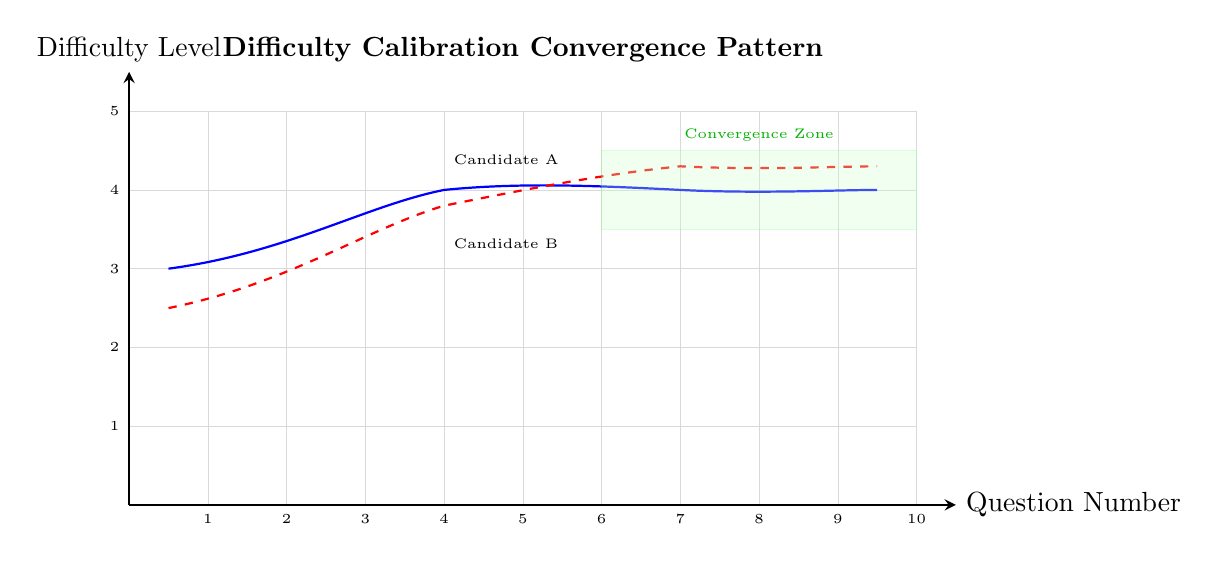
\begin{tikzpicture}[
    scale=1.0,
    axis/.style={->, >=stealth, thick},
    grid/.style={gray!30, very thin},
    plot/.style={thick, blue},
    plot2/.style={thick, red, dashed}
]

% Draw grid
\draw[grid] (0,0) grid (10,5);

% Axes
\draw[axis] (0,0) -- (10.5,0) node[right] {Question Number};
\draw[axis] (0,0) -- (0,5.5) node[above] {Difficulty Level};

% Axis labels
\foreach \x in {1,2,...,10}
    \draw (\x,0) node[below] {\tiny \x};
\foreach \y in {1,2,3,4,5}
    \draw (0,\y) node[left] {\tiny \y};

% Plot convergence pattern (example: starts at 3, converges to 4)
\draw[plot] (0.5,3) .. controls (2,3.2) and (3,3.8) .. (4,4) .. controls (5,4.1) and (6,4.05) .. (7,4) .. controls (8,3.95) and (9,4) .. (9.5,4);
\draw[plot2] (0.5,2.5) .. controls (2,2.8) and (3,3.5) .. (4,3.8) .. controls (5,4) and (6,4.2) .. (7,4.3) .. controls (8,4.25) and (9,4.3) .. (9.5,4.3);

% Add labels
\node[above right] at (4,4.2) {\tiny Candidate A};
\node[below right] at (4,3.5) {\tiny Candidate B};

% Add convergence zone
\draw[green!50, fill=green!20, opacity=0.3] (6,3.5) rectangle (10,4.5);
\node[green!70!black] at (8,4.7) {\tiny Convergence Zone};

% Title
\node[above] at (5,5.5) {\textbf{Difficulty Calibration Convergence Pattern}};

\end{tikzpicture}



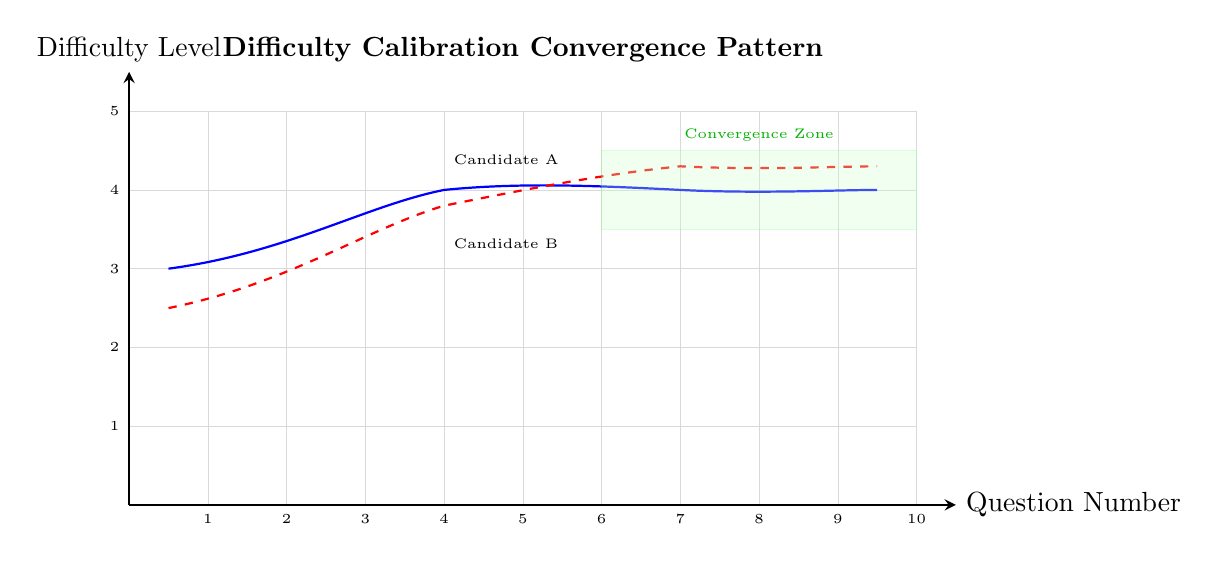
\begin{tikzpicture}[
    scale=1.0,
    axis/.style={->, >=stealth, thick},
    grid/.style={gray!30, very thin},
    plot/.style={thick, blue},
    plot2/.style={thick, red, dashed}
]

% Draw grid
\draw[grid] (0,0) grid (10,5);

% Axes
\draw[axis] (0,0) -- (10.5,0) node[right] {Question Number};
\draw[axis] (0,0) -- (0,5.5) node[above] {Difficulty Level};

% Axis labels
\foreach \x in {1,2,...,10}
    \draw (\x,0) node[below] {\tiny \x};
\foreach \y in {1,2,3,4,5}
    \draw (0,\y) node[left] {\tiny \y};

% Plot convergence pattern (example: starts at 3, converges to 4)
\draw[plot] (0.5,3) .. controls (2,3.2) and (3,3.8) .. (4,4) .. controls (5,4.1) and (6,4.05) .. (7,4) .. controls (8,3.95) and (9,4) .. (9.5,4);
\draw[plot2] (0.5,2.5) .. controls (2,2.8) and (3,3.5) .. (4,3.8) .. controls (5,4) and (6,4.2) .. (7,4.3) .. controls (8,4.25) and (9,4.3) .. (9.5,4.3);

% Add labels
\node[above right] at (4,4.2) {\tiny Candidate A};
\node[below right] at (4,3.5) {\tiny Candidate B};

% Add convergence zone
\draw[green!50, fill=green!20, opacity=0.3] (6,3.5) rectangle (10,4.5);
\node[green!70!black] at (8,4.7) {\tiny Convergence Zone};

% Title
\node[above] at (5,5.5) {\textbf{Difficulty Calibration Convergence Pattern}};

\end{tikzpicture}



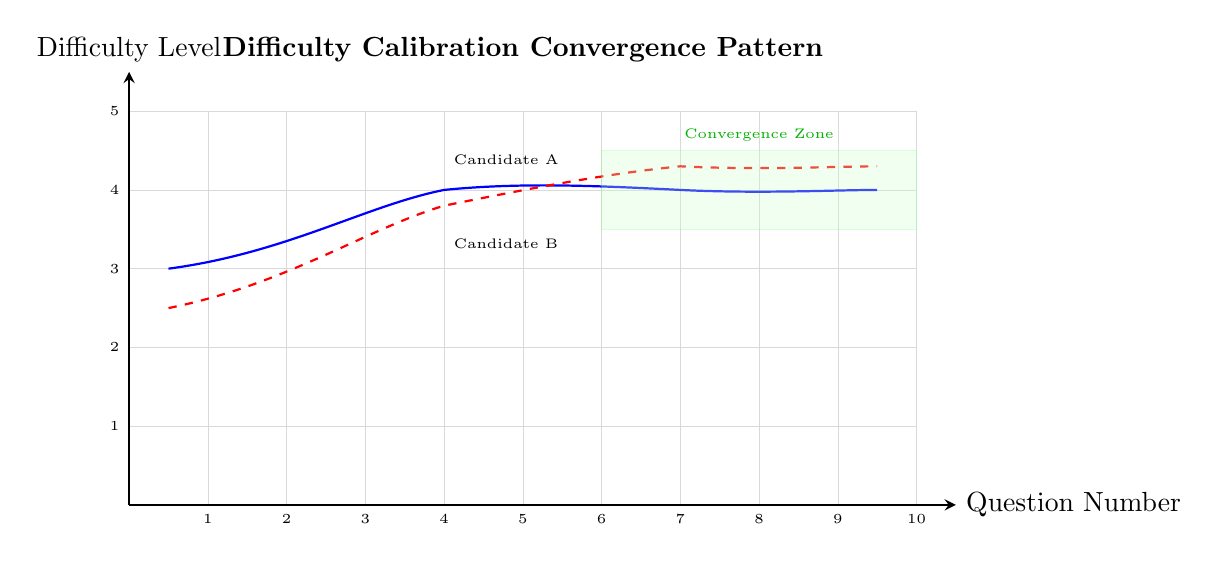
\begin{tikzpicture}[
    scale=1.0,
    axis/.style={->, >=stealth, thick},
    grid/.style={gray!30, very thin},
    plot/.style={thick, blue},
    plot2/.style={thick, red, dashed}
]

% Draw grid
\draw[grid] (0,0) grid (10,5);

% Axes
\draw[axis] (0,0) -- (10.5,0) node[right] {Question Number};
\draw[axis] (0,0) -- (0,5.5) node[above] {Difficulty Level};

% Axis labels
\foreach \x in {1,2,...,10}
    \draw (\x,0) node[below] {\tiny \x};
\foreach \y in {1,2,3,4,5}
    \draw (0,\y) node[left] {\tiny \y};

% Plot convergence pattern (example: starts at 3, converges to 4)
\draw[plot] (0.5,3) .. controls (2,3.2) and (3,3.8) .. (4,4) .. controls (5,4.1) and (6,4.05) .. (7,4) .. controls (8,3.95) and (9,4) .. (9.5,4);
\draw[plot2] (0.5,2.5) .. controls (2,2.8) and (3,3.5) .. (4,3.8) .. controls (5,4) and (6,4.2) .. (7,4.3) .. controls (8,4.25) and (9,4.3) .. (9.5,4.3);

% Add labels
\node[above right] at (4,4.2) {\tiny Candidate A};
\node[below right] at (4,3.5) {\tiny Candidate B};

% Add convergence zone
\draw[green!50, fill=green!20, opacity=0.3] (6,3.5) rectangle (10,4.5);
\node[green!70!black] at (8,4.7) {\tiny Convergence Zone};

% Title
\node[above] at (5,5.5) {\textbf{Difficulty Calibration Convergence Pattern}};

\end{tikzpicture}



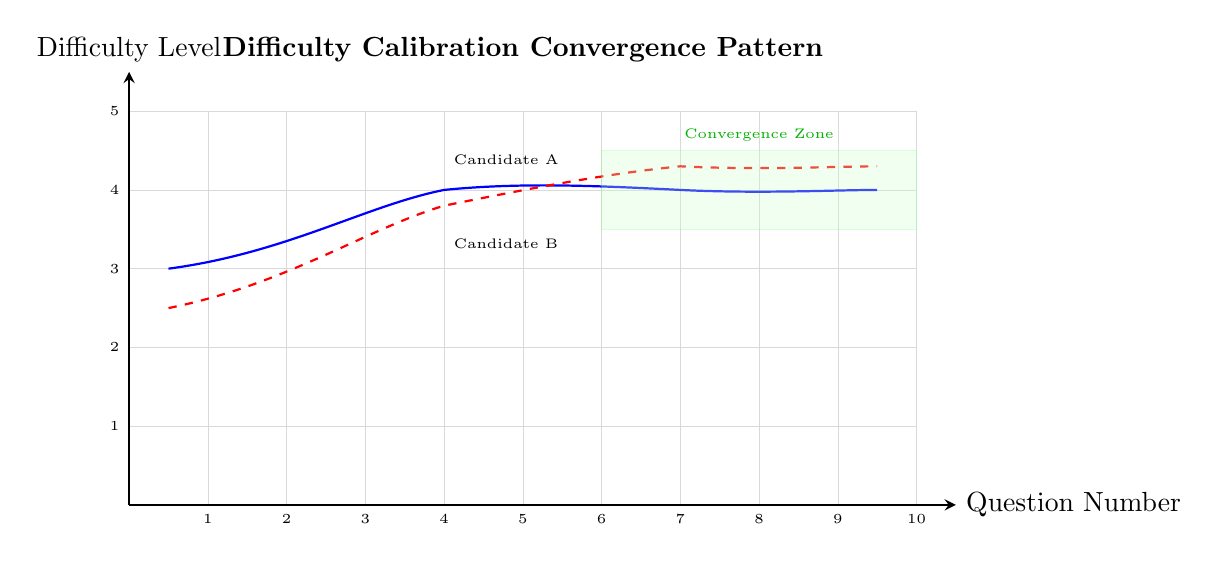
\begin{tikzpicture}[
    scale=1.0,
    axis/.style={->, >=stealth, thick},
    grid/.style={gray!30, very thin},
    plot/.style={thick, blue},
    plot2/.style={thick, red, dashed}
]

% Draw grid
\draw[grid] (0,0) grid (10,5);

% Axes
\draw[axis] (0,0) -- (10.5,0) node[right] {Question Number};
\draw[axis] (0,0) -- (0,5.5) node[above] {Difficulty Level};

% Axis labels
\foreach \x in {1,2,...,10}
    \draw (\x,0) node[below] {\tiny \x};
\foreach \y in {1,2,3,4,5}
    \draw (0,\y) node[left] {\tiny \y};

% Plot convergence pattern (example: starts at 3, converges to 4)
\draw[plot] (0.5,3) .. controls (2,3.2) and (3,3.8) .. (4,4) .. controls (5,4.1) and (6,4.05) .. (7,4) .. controls (8,3.95) and (9,4) .. (9.5,4);
\draw[plot2] (0.5,2.5) .. controls (2,2.8) and (3,3.5) .. (4,3.8) .. controls (5,4) and (6,4.2) .. (7,4.3) .. controls (8,4.25) and (9,4.3) .. (9.5,4.3);

% Add labels
\node[above right] at (4,4.2) {\tiny Candidate A};
\node[below right] at (4,3.5) {\tiny Candidate B};

% Add convergence zone
\draw[green!50, fill=green!20, opacity=0.3] (6,3.5) rectangle (10,4.5);
\node[green!70!black] at (8,4.7) {\tiny Convergence Zone};

% Title
\node[above] at (5,5.5) {\textbf{Difficulty Calibration Convergence Pattern}};

\end{tikzpicture}

